\documentclass[a4paper,12pt]{article}
\usepackage[MeX]{polski}
\usepackage[utf8]{inputenc}
\usepackage{graphicx}

%opening
\title{Tabia Charles}
\author{}

\begin{document}

\maketitle
\centering
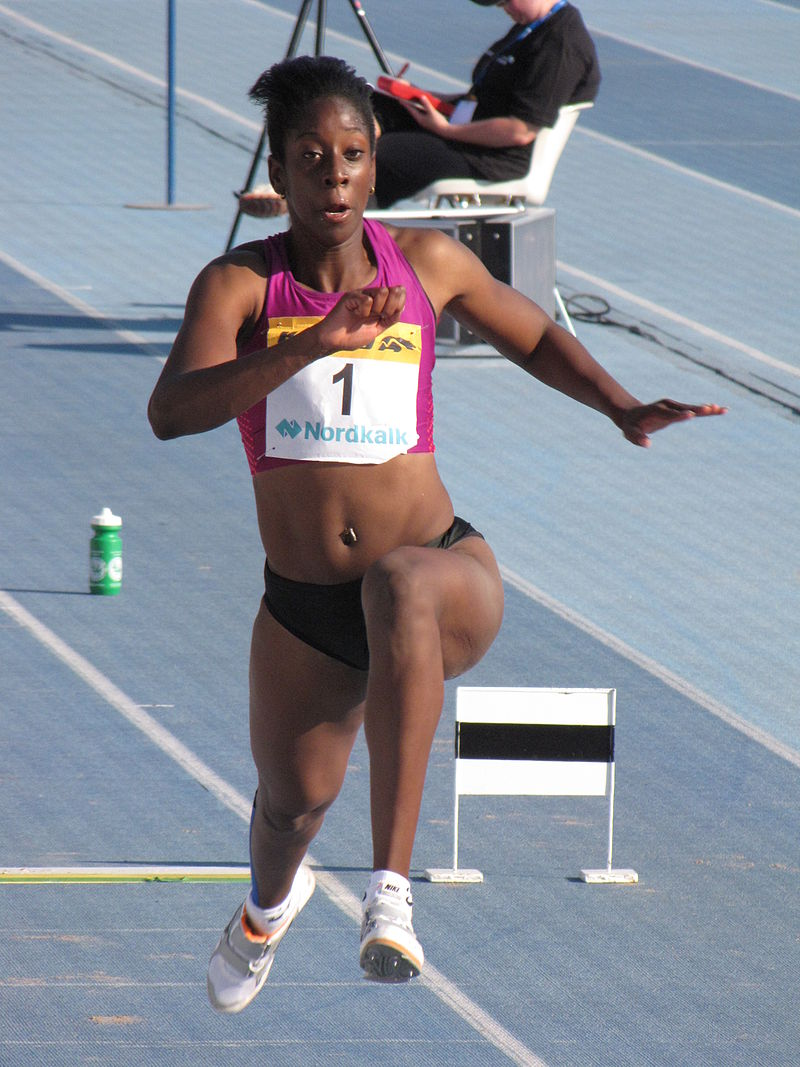
\includegraphics[scale=0.50]{Tabia-Charles.jpg}
\begin{itemize}
\item
Tabia Hasina Charles (ur. 6 kwietnia 1985 w Toronto) --- kanadyjska lekkoatletka specjalizująca się w trójskoku oraz skoku w dal.
\item Reprezentowała Kanadę podczas igrzysk olimpijskich w 2008 roku zajmując w tych zawodach dziesiąte miejsce wśród skoczkiń w dal. W 2010 odpadła w eliminacjach skoku w dal na halowych mistrzostwach świata, a na koniec sezonu wywalczyła dwa brązowe medale igrzysk Wspólnoty Narodów w konkursie trójskoku i skoku w dal.
\item Wielokrotna medalistka mistrzostw Kanady w różnych konkurencjach (podczas czempionatu w 2010 roku wygrała skok w dal i trójskok).

\item Rekordy życiowe: skok w dal --- hala: 6,60; stadion: 6,82; trójskok – hala 14,02; stadion 13,99. Dwa ostatnie wyniki są aktualnymi rekordami Kanady.

\end{itemize}



\begin{table}
\begin {tabular}{cccccc}
Rok & Imprez & Miejsce & konkurencja & Lokata & Wynik\\
\hline
2008 & Igrzyska olimpijskie &  Pekin & skok w dal & 10. miejsce & 6,47\\
\hline
2010 & Halowe mistrzostwa świata & Doha & skok w dal & el. --- 15. miejsce & 6,32\\
\hline
2010 & Igrzyska Wspólnoty Narodów & Nowe Delhi & trójskok & 3.miejwsce & 13,84\\
\hline
2010 & Igrzyska Wspólnoty Narodów & Nowe Delhi & skok w dal & 3.miejwsce & 6,44\\

\end{tabular}
\caption{Osiągnięcia}
\end{table}




\end{document}
